\documentclass[10pt,aspectratio=169]{beamer}
\usetheme{default}\usecolortheme{seagull}\setbeamertemplate{navigation symbols}{}\setbeamertemplate{footline}[frame number]
\usepackage[T1]{fontenc}\usepackage{mathptmx}\usepackage{booktabs}\usepackage{graphicx}\usepackage{tabularx}\usepackage{ragged2e}
\setbeamerfont{title}{size=\large,series=\bfseries}\setbeamerfont{frametitle}{size=\normalsize,series=\bfseries}
\setbeamercolor{frametitle}{fg=black}\setbeamercolor{title}{fg=black}
\title{The ANNNI phase diagram under two classes of error}
\subtitle{What depolarizing noise and coherent drift each do to a phase boundary, and what recovers it}
\author{Matthew Stanley Leibel \quad TrueLoop Compute (NEOTECH Inc.)}
\date{QSITE 2026 Quantum Coalition, Scientific Track}
\begin{document}
\begin{frame}\titlepage
\vspace{-6pt}\centering\small\textit{Depolarizing noise fades a phase diagram. Coherent drift moves it. Different mitigations fix each, and together they separate what calibration can recover from what decoherence costs.}
\end{frame}

\begin{frame}{1. The model, the observable, and the clean diagram}
\begin{columns}[T]\begin{column}{0.5\textwidth}
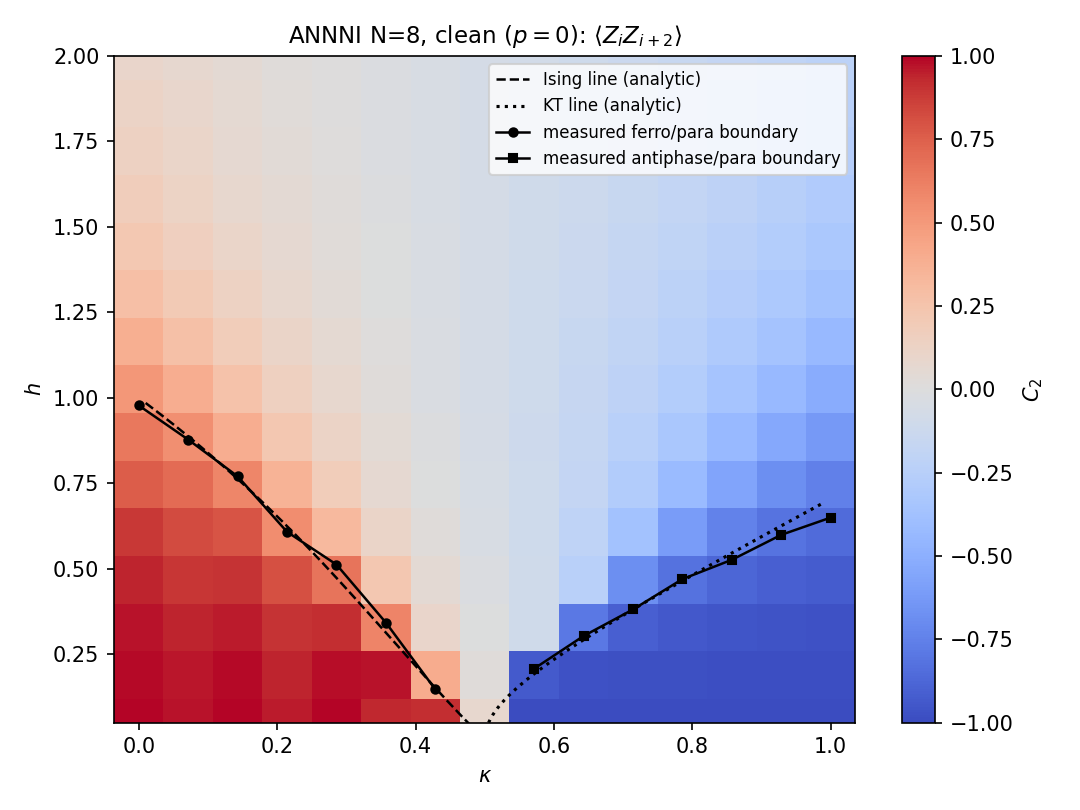
\includegraphics[width=\textwidth]{../figures/phase_diagram_p0.png}
\end{column}\begin{column}{0.48\textwidth}\small
$H=-\sum Z_iZ_{i+1}+\kappa\sum Z_iZ_{i+2}-h\sum X_i$, $N=8$, periodic, $15\times15$ grid.\\[6pt]
Observable: $C_2=\frac1N\sum\langle Z_iZ_{i+2}\rangle$. $+1$ ferromagnet, $-1$ antiphase ($\uparrow\uparrow\downarrow\downarrow$), $\approx0$ paramagnet. Symmetry-safe at finite size.\\[6pt]
Thresholds fixed once on the analytic lines and never changed.\\[6pt]
Ferro/para at $\kappa=0.29$: $h^*=0.512$ (Ising line 0.473).\\ Antiphase/para at $\kappa=0.71$: $h^*=0.381$ (KT line 0.381).\\[6pt]
$\kappa=0.5$: multicritical, no ordered reference, handled separately.
\end{column}\end{columns}
\end{frame}

\begin{frame}{2. Preparation and the two error classes}
\small
\textbf{Circuit.} Hamiltonian-variational ansatz from $|+\rangle^{\otimes N}$: four layers of $e^{-ig_1\sum ZZ_{nn}}e^{-ig_2\sum ZZ_{nnn}}e^{-ib\sum X}$, 12 parameters, 128 CNOTs. L-BFGS with adjoint gradients, warm-started from the paramagnet. Median energy error $4\times10^{-5}$; $C_2$ within 0.05 of exact diagonalization at 95\% of points.\\[8pt]
\textbf{Error class 1, the track's question.} \texttt{DepolarizingChannel}$(p)$ on the target after every CNOT, $p=0.01$ and $0.05$, on PennyLane \texttt{default.mixed}, all 225 points.\\[8pt]
\textbf{Error class 2, what every processor also has.} Every $RX$ angle $\times(1+\epsilon_i)$, every $RZZ$ angle $\times(1+\delta_k)$, drifting across the scan: static offset plus wander, common-mode plus independent, RMS 3\% and 6\%.\\[8pt]
\textbf{Two mitigations.} Rescale by a reference point (measure the decay). Or hold the angles in-band: five probe circuits per cycle feeding a per-channel controller that corrects only above the noise floor and learns each slope from its own motion.
\end{frame}

\begin{frame}{3. Depolarizing is amplitude loss}
\begin{columns}[T]\begin{column}{0.56\textwidth}
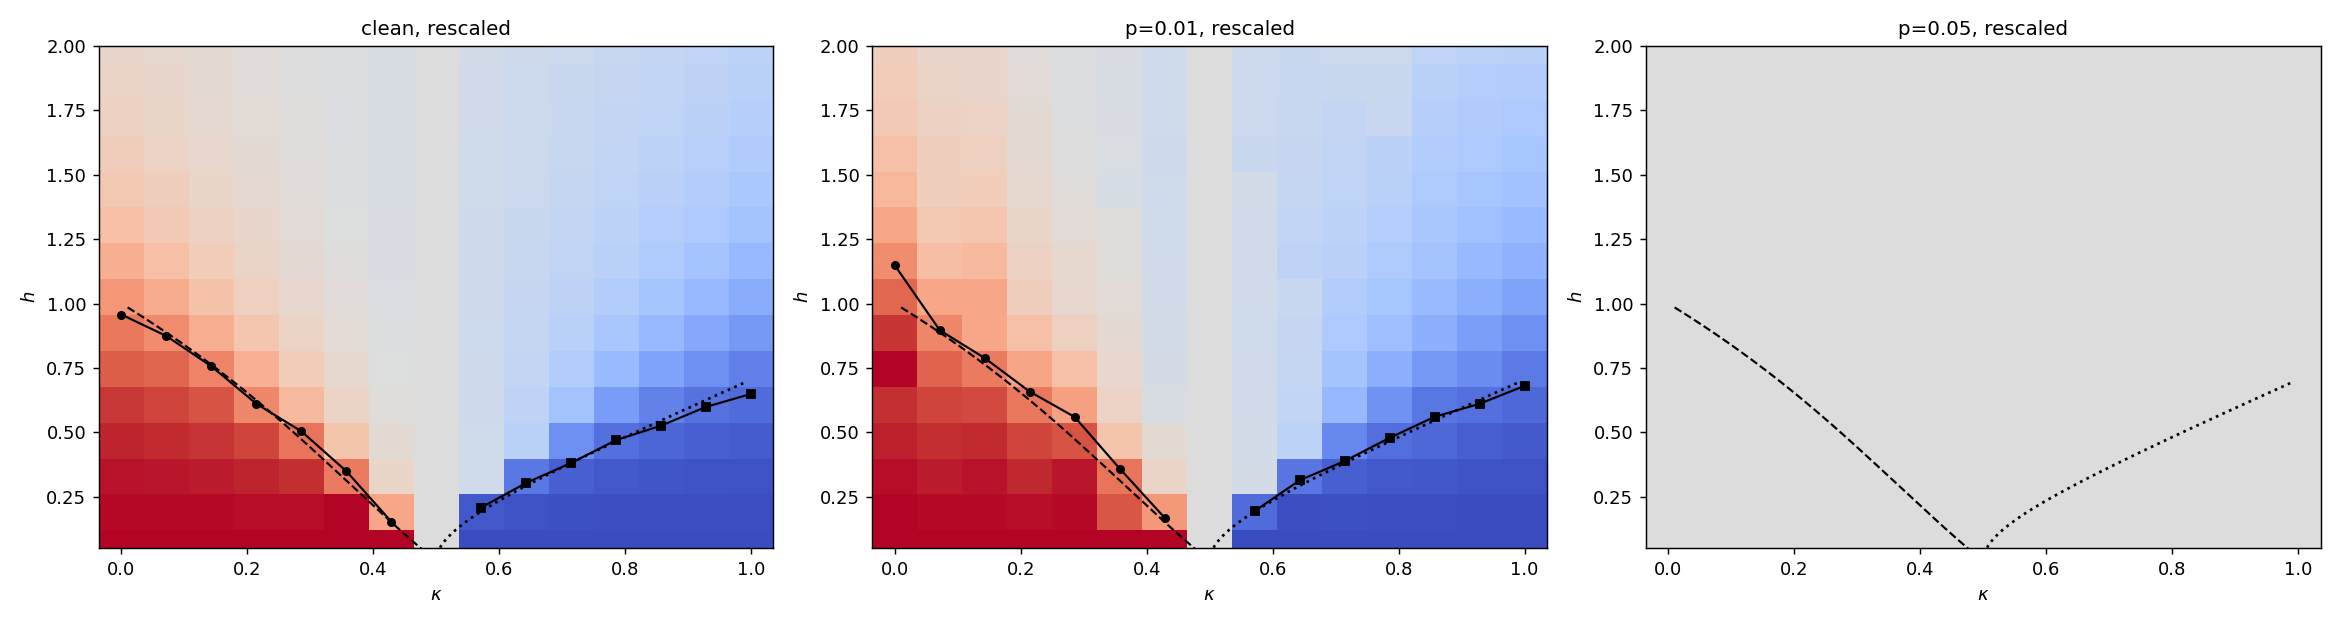
\includegraphics[width=\textwidth]{../figures/depolarizing_rescaled.png}
\end{column}\begin{column}{0.42\textwidth}\small
Deep-ordered signal: 0.92 $\to$ 0.48 at $p=0.01$, 0.05 at $p=0.05$.\\[4pt]
Fixed threshold: every ordered point lost at both levels (24.9\%).\\[4pt]
Rescaled by the $h=0.05$ reference: $p=0.01$ recovers to 1.3\% misclassified; ferro/para $0.504\to0.559$, antiphase/para $0.381\to0.388$. $p=0.05$: nothing recovers it.\\[4pt]
\textbf{Most robust: the antiphase} (0.60 of clean vs 0.37 for the ferromagnet at $p=0.01$). The ferromagnet is built with more $X$ rotation late in the circuit, after the CNOTs that carry the noise. The opposite of the naive guess.\\[4pt]
What matters is $p\times$depth: 256 CNOTs lose the phases at $p=0.01$ outright.
\end{column}\end{columns}
\end{frame}

\begin{frame}{4. Coherent drift is shape distortion}
\begin{columns}[T]\begin{column}{0.58\textwidth}
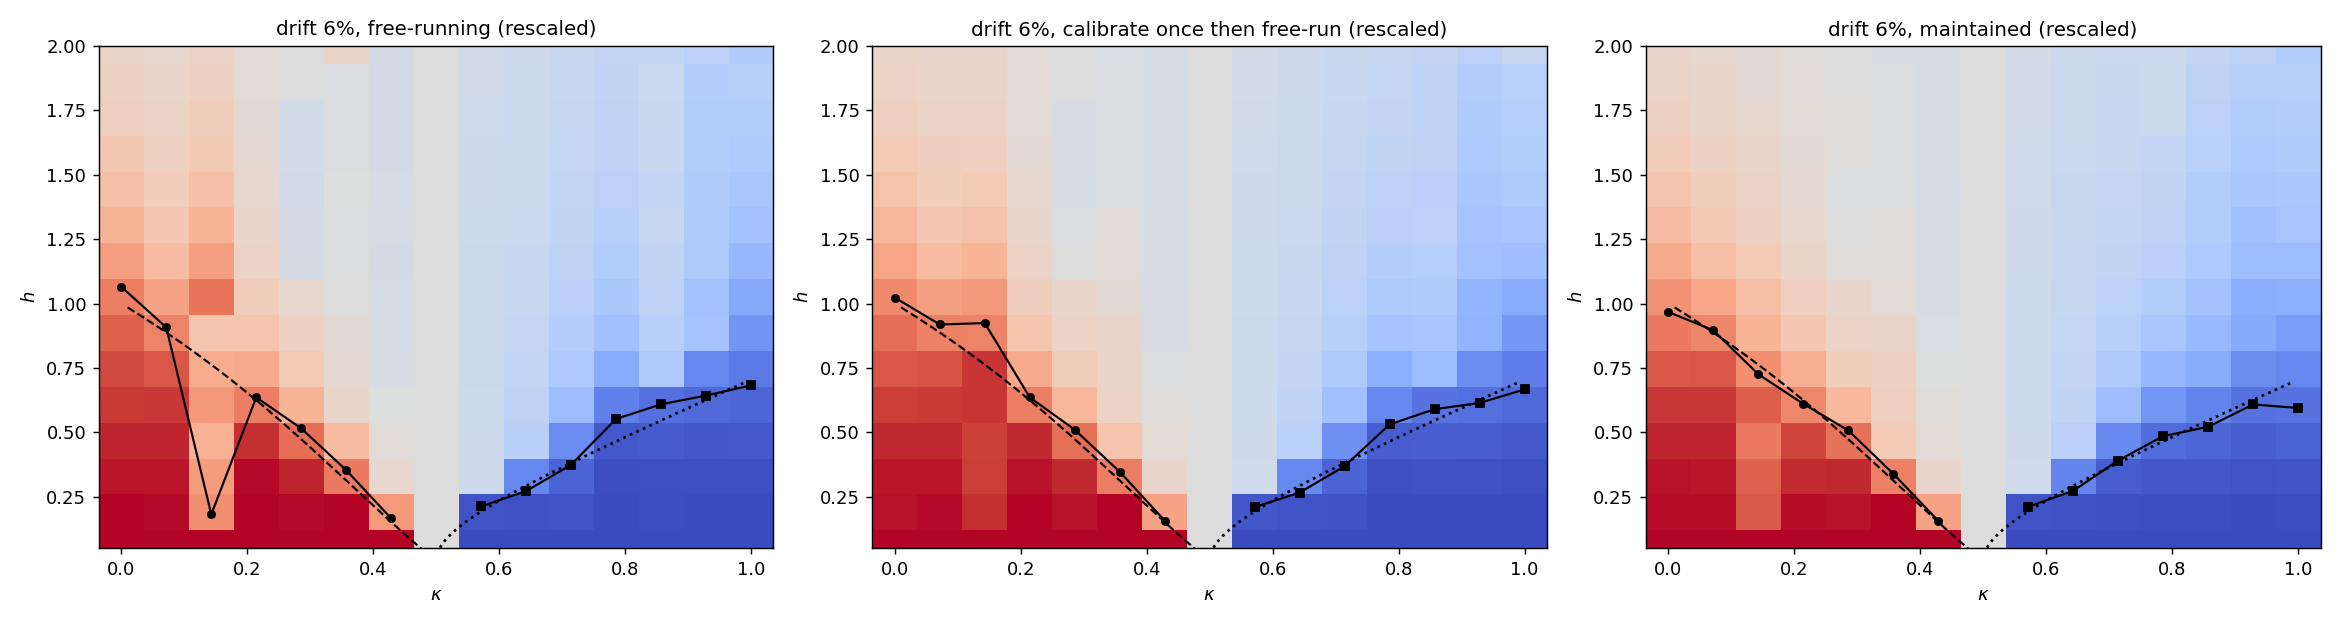
\includegraphics[width=\textwidth]{../figures/drift_free_vs_maintained.png}
\end{column}\begin{column}{0.4\textwidth}\small
Signed and first order: $+10\%$ over-rotation moves $C_2$ by $-0.056$, under-rotation the other way. Boundaries move; rescaling cannot help.\\[6pt]
6\% drift, free-running: mean shift 0.075, one excursion of 0.58, 4.4\% misclassified.\\[6pt]
Calibrate once, then free-run: 0.037 (the static half).\\[6pt]
Maintained in-band: 0.015, 1.8\% misclassified, 80\% of the shift removed. At 3\%: 0.016 $\to$ 0.007.\\[6pt]
The ferromagnetic boundary moves $3\times$ more than the antiphase boundary: $C_2$ is steeper there.
\end{column}\end{columns}
\end{frame}

\begin{frame}{5. What recovers what, and at what cost}
\footnotesize
\begin{tabularx}{\textwidth}{>{\RaggedRight\arraybackslash}p{0.40\textwidth} >{\RaggedRight\arraybackslash}p{0.13\textwidth} >{\RaggedRight\arraybackslash}p{0.12\textwidth} >{\RaggedRight\arraybackslash}X}\toprule
Arm (rescaled boundaries, $N=8$) & misclassified & mean $|\Delta h^*|$ & operations\\\midrule
depolarizing $p=0.01$ & 1.3\% & 0.035 & rescaling, no circuits\\
depolarizing $p=0.05$ & 24.9\% & none & unrecoverable\\
drift 6\%, free-running & 4.4\% & 0.075 & none\\
drift 6\%, calibrate once at the start & 1.3\% & 0.037 & one sweep\\
drift 6\%, re-optimize the VQE at every point & 0.0\% (sub-grid) & & about 36,000 circuits per point\\
drift 6\%, maintained in-band & 1.8\% & 0.015 & 5 probe circuits per cycle\\
drift 6\% and $p=0.01$ together, free / maintained, measured against the depolarizing-only diagram & 3.6\% / 0.4\% & 0.070 / 0.038 & boundaries land on the depolarizing-only ones\\
\bottomrule\end{tabularx}\\[12pt]
\small Under both errors, maintenance returns the diagram to its depolarizing-only form: the incoherent part is isolated, and it is the only part left.
\end{frame}

\begin{frame}{6. Continuous, unsupervised, in real time}
\begin{columns}[T]\begin{column}{0.6\textwidth}
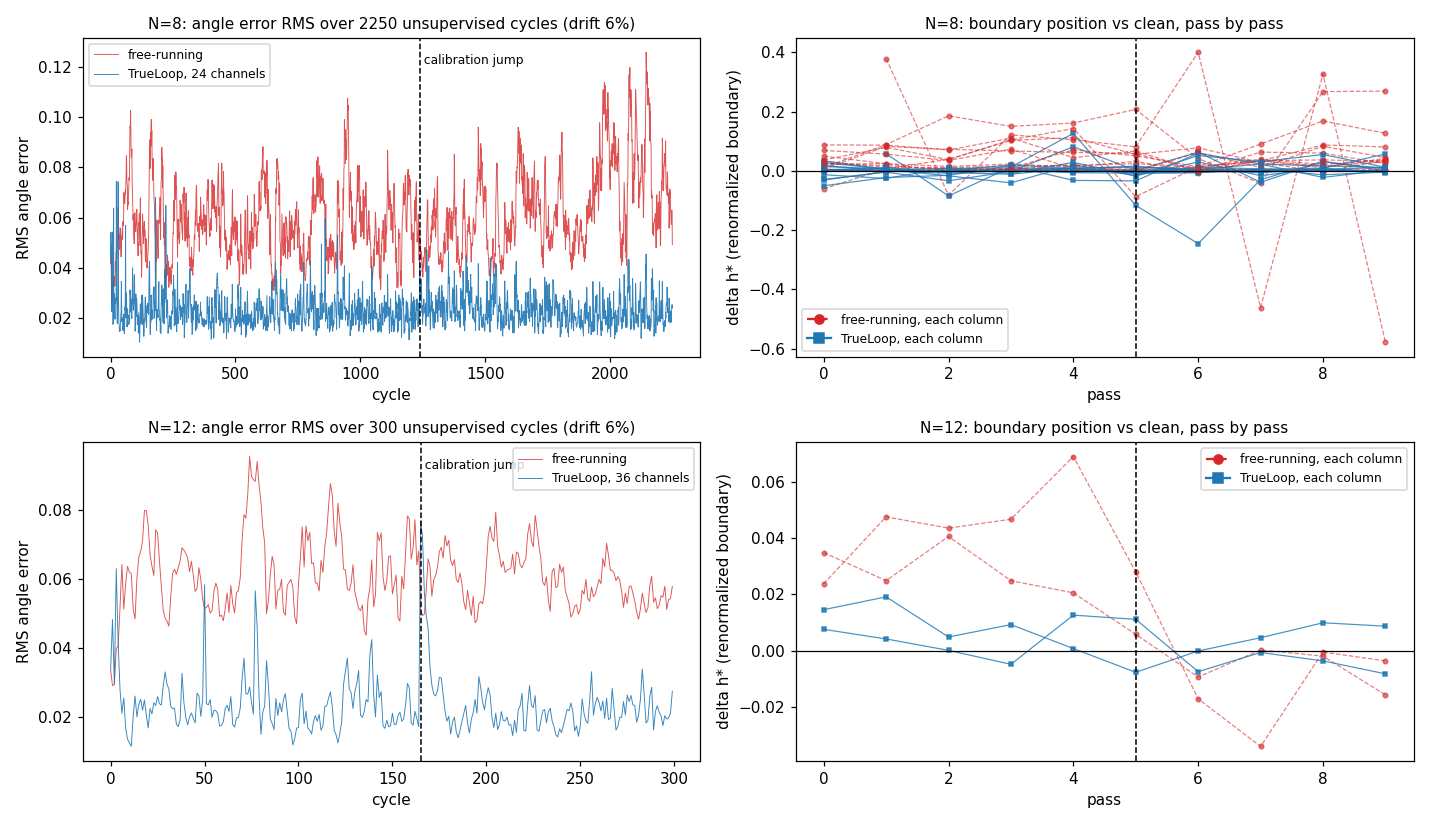
\includegraphics[width=\textwidth]{../figures/continuous_operation.png}
\end{column}\begin{column}{0.38\textwidth}\small
Ten passes, 2,250 cycles, 6\% drift, every offset redrawn at pass 5, nobody intervening.\\[6pt]
$N=8$, 24 channels: residual 0.062 $\to$ 0.024 every pass; boundary std 0.051 $\to$ 0.020; jump absorbed in 3 cycles; host 47\,$\mu$s per cycle.\\[6pt]
$N=12$, 36 channels: 0.062 $\to$ 0.025; std 0.025 $\to$ 0.007; 76\,$\mu$s per cycle. Linear in channels.\\[6pt]
Free-running walks away by the last pass. The maintained diagram does not move.
\end{column}\end{columns}
\end{frame}

\begin{frame}{7. Complexity decoupled from the state}
\begin{columns}[T]\begin{column}{0.58\textwidth}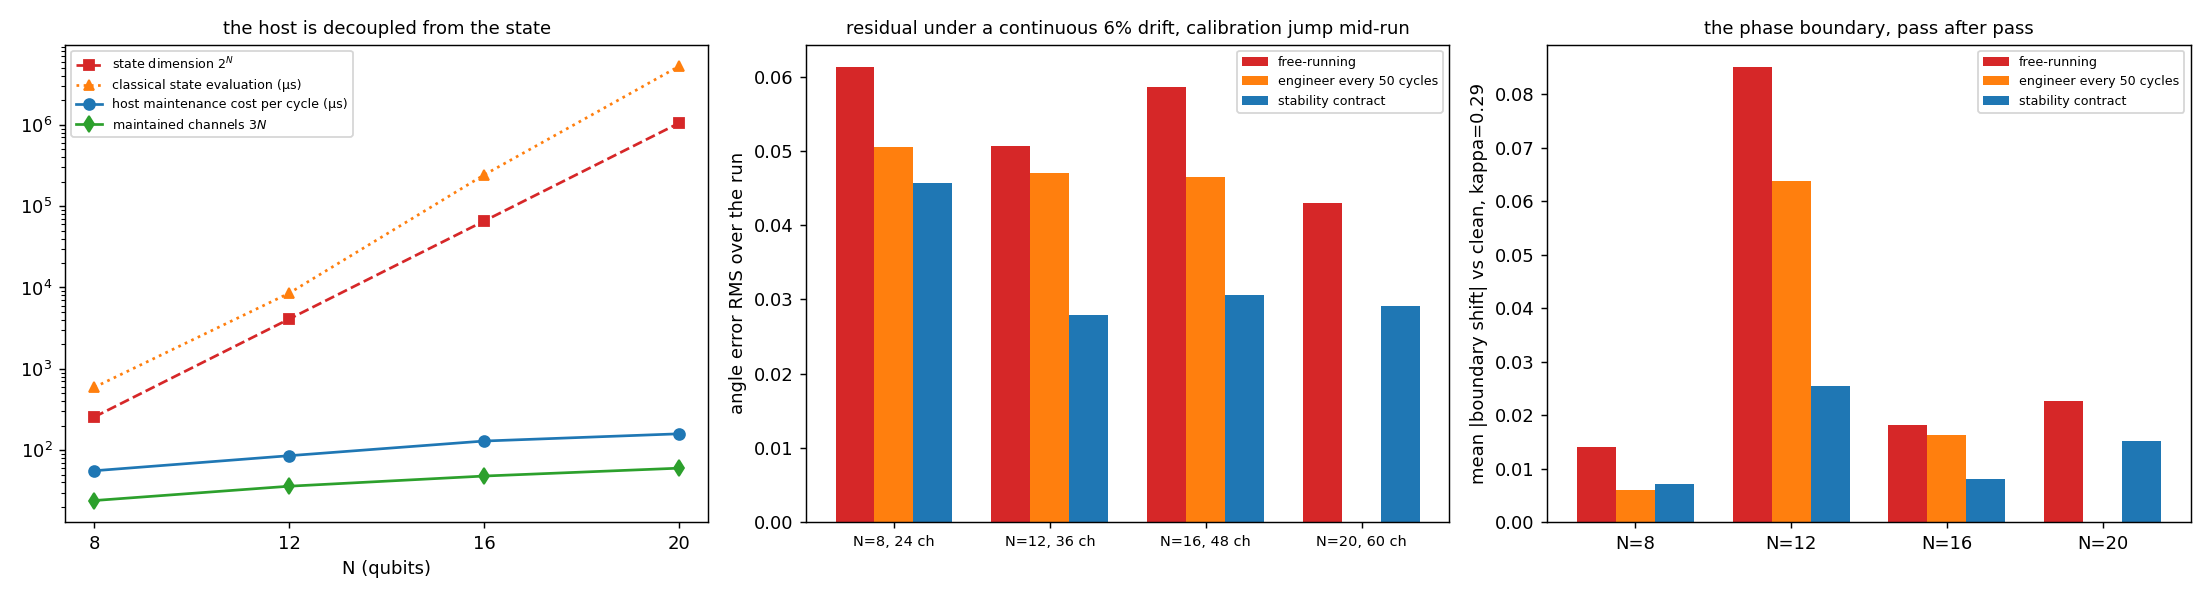
\includegraphics[width=\textwidth]{../figures/decoupling.png}\end{column}\begin{column}{0.4\textwidth}\footnotesize
Two things keep continuous hardware in a lab: a person recalibrating it on a schedule, which cannot follow a wander faster than the schedule; or a host reconstructing its state, which costs $n^2$ memory and cannot reach high dimension. The contract does neither: $3N$ channels from one read, while the state has $2^N$ amplitudes.\\[5pt]
$N=8\to20$: state dimension $\times$4,096; classical state evaluation 1\,ms $\to$ 5.2\,s; host maintenance cost 56 $\to$ 159\,$\mu$s, linear at 2.6\,$\mu$s per channel.\\[5pt]
Three arms on the same scan: free-running, an engineer every 50 cycles, the contract. At every size the contract holds the boundary tighter than the scheduled engineer; at $N=12$, three times tighter (0.085 / 0.064 / 0.025).\\[5pt]
The host never touches the state, so its burden does not grow with it. That is what lets a hybrid system scale.
\end{column}\end{columns}
\end{frame}

\begin{frame}{8. Interpretation, limitations, what is next}
\small
\textbf{In the model's language.} Depolarizing shortens every correlation length uniformly: order parameters shrink, boundaries stay, a ratio observable sees them until the correlation length is below two sites. Coherent drift changes the effective Hamiltonian the circuit prepares, shifting where frustration and field balance: the boundary really moves. Rescaling fixes one, maintenance fixes the other.\\[8pt]
\textbf{Not resolved.} The floating phase, at $N=8$; the two poorly converged points near $\kappa\approx0.6$ sit exactly there.\\[8pt]
\textbf{Limitations.} $N=8$ periodic; noise after CNOTs only; the wander speed sets the maintenance floor at 0.4; the eight-layer circuits are exact at $N=12$ and at their limit by $N=16$. One product boundary found: with declared signs and a low-SNR probe the controller mis-identified channels and held them; letting it learn the signs fixed it.\\[8pt]
\textbf{Everything reproduces.} Executed notebook, PennyLane grids, cached data, code, and the maintenance layer's evaluation build are in the package.
\end{frame}
\end{document}
